\documentclass{iitbthesis}
\usepackage[latin1]{inputenc}
\usepackage{amsmath}
\usepackage{amsfonts}
\usepackage{amssymb}
\usepackage{makeidx}
\usepackage{graphicx}
\usepackage{multirow}
\usepackage{epstopdf}
\usepackage{epsfig}
\usepackage{empheq}
\usepackage{hyperref}
\usepackage{bm}
\usepackage{url}
\newcommand*\widefbox[1]{\fbox{\hspace{2em}#1\hspace{2em}}}
\usepackage{appendix}
\usepackage[section]{placeins}  %to stop floating of figures b/w sections
\usepackage[a4paper, vmargin={5cm,3cm}, hmargin={3cm,2cm}]{geometry}

%%%%%%%%%%%%%%%%%%%%%%%%%%%%%%%%%%%%%%%%%%%%%%%%%%%%%
\usepackage{vmargin}
\setpapersize{A4}
\setmarginsrb{30mm}{15mm}{20mm}{22mm}{3mm}{12mm}{3mm}{10mm}
%%%%%%%%%%%%%%%%%%%%%%%%%%%%%%%%%%%%%%%%%%%%%%%%%%%%%
\setlength{\parsep}{20pt}
\setlength{\textwidth}{160mm}
\setlength{\textheight}{245mm}
\usepackage{fancyhdr}
\pagestyle{fancy}
\lhead{}
\chead{}
\rhead{\textit{Development and testing of standard compliant Phasor Measurement Unite}}
\lfoot{\textit{Electrical Engineering Dept.}}
\cfoot{\thepage}
\rfoot{\textit{IIT Bombay}}
\renewcommand{\headrulewidth}{0pt}
\renewcommand{\footrulewidth}{0pt}
\author{Rathin Dholakia}

%%%%%%%%%%%%%%%%%%%%%%%%%%%%%%%%%%%%%%%%%%%%%%%%%%%%%
\begin{document}
\thispagestyle{empty}
\begin{center}
%\vspace*{30pt}
\huge
\textbf{Design and Development of Phasor Measurement Unit and it's compliance testing using mini-FSS}\\
\bigskip
\bigskip
%\bigskip
%\bigskip
%\bigskip
\normalsize
\textit{Submitted in partial fulfillment of the requirements\\
                for  the degree of 
 }\\
\vspace*{0.8cm}
\textbf{MASTER OF TECHNOLOGY}\\
\textbf{(Power Electronics $ \& $ Power Systems)}\\
\vspace*{0.8cm}
\textit{by}\\
\vspace*{0.8cm}
\textbf{Rathin Dholakia \\(143076001)}\\
\vspace*{0.8cm}
\textit{under the guidance of}\\
\textbf{Prof. Mukul C. Chandorkar}\\
\vspace*{0.8cm}
\begin{figure}[h!]
 \centering
 \includegraphics[trim=1cm 1cm 5cm 12.5cm, clip=true, width=4cm]{chapter0_initial/logo}
\end{figure}
\bigskip
\bigskip
\large
\textbf{Department of Electrical Engineering}\\
\bigskip
\textbf{INDIAN INSTITUTE OF TECHNOLOGY BOMBAY}\\
\bigskip
\textbf{June 2017}
\end{center}

\normalsize
 



% Dedication
\newpage
\thispagestyle{empty}
\vspace*{200pt}
\begin{center}
 \large

 \textit{
Dedicated to\\
\bigskip
 Parents \& Friends}
\end{center}
\normalsize
%\chapter*{\center Dissertation Approval Certificate}
%\addcontentsline{toc}{chapter}{Abstract}

%%USING A NEW TITLE PAGE
\thispagestyle{empty}
%\vspace{0.3in}

%\hfill

%\centerline{\textbf{\large Approval Sheet}}

%\vspace{1cm}

This dissertation entitled \textbf{Thesis Title} by
\textbf{AUTHOR NAME} (Roll No: AUTHOR'S ROLL NO.) is approved for the degree of \textbf{Master of Technology} in Electrical Engineering with specialization in \textbf{Power Electronics and Power Systems} from \textbf{Indian Institute of Technology Bombay}, India.


\vspace{1.5cm}


\begin{tabular}{llc}
\hspace{4cm} & \hspace{4cm} & \hspace{1.5cm} Examiners \hspace{1.5cm} \\ \\
             &              & \hrulefill \\ \\ \\
             &              & \hrulefill \\ \\


  \hspace{1cm} Supervisor &              & Chairman   \\ \\
   \hrulefill&              &  \hrulefill \\ \\


Date:\hrulefill & & \\ \\
Place: \hrulefill & & \\
\end{tabular}


%\input{chapter0_initial/Declaration.tex}
%\pagenumbering{roman}
\chapter*{Acknowledgement}
 Write your acknowledgements here
\vspace*{30pt}
\begin{flushright}
\textbf{AUTHOR NAME}
\end{flushright}
%\chapter*{Abstract}
\singlespace
\textbf{
Write your abstract here
}
\doublespace

\tableofcontents
\listoffigures
\listoftables

\chapter{Introduction}
\pagenumbering{arabic}  % 1, 2, 3, 4, ...
\setcounter{page}{1}

Electric energy has become most important source of energy and is widely used resource in present time, with ever increasing demand of the resource it becomes more and more difficult to maintain the system and Power System is no exception. Power System has become an complex entity and has gone beyond the limit of manual operattion and control which makes automation and "smart" control imparitive. This creates demand for new set of measurement, operation and control tools. Out of this tools measurement tools are the most fundaental building block of the modern power system which is also know populalry as "smart grid". They are the "eyes" and "ears" in the system to the centralized operating-control-corrective brain system.  

In power system active power and frequency are the most important parameters to be monitored, flow of active power is decided by the phase angle of voltage between buses. Flow of active power decides the structure of network (transmission lines, capacity of devices etc) and hence accurate measurement of it has been of great interest since 1980s.\cite{agphadkebook}. Conventionally relative phase angle between buses in the network, due to limitation of telecommunication links, computational power and the economic pheasibility. This method(s) were slow, fairly accurate and dependent on a tones of heavy manual calcualtion. 
After advancements in communition channels and their speed \& reliability, better computation and satelite availability, trend of absolute phase difference measurement came in to existance.   
\section{Phasors, Synchrophasors and PMUs}
\subsection{Phasors: Defination}
In Physics and engineering, \textit{phasor} is a complex number representing a sinusoidal quantity whose amplitude (A), angular velocity ($\omega$) and initial phase ($\phi$) are time-invarient.It is an analytic representation which decomposes sine function in to product of complex constants and a factor which encapsulates the frequency and time dependence.
\section{Chapter 1 Section 2}

\chapter{Literature Survey}
Literature survey is split in two parts, one that covers the design and development of PMU  and other about testing procedures for standard compliant testing.

A survey was made of the PMUs designed developed elsewhere in the academia for knowing the experience, best practices and targeted performance and ways of implementation. Few PMU implementation worth noting here are as follows:

\subsubsection{GRIDTrak PMU} It is one of the oldest synchrophasor implementation, a PMU developed by Baltimore University \cite{dotta2014teaching} was aimed towards teaching measurement of AC synchrophasors' frequency, amplitude and angle. It used set of Op-amp and voltage comparators to convert input sine to square and was using accurate timer to measure the distance between two zero crossings. An accurate timer was also keeping track of offset between 1PPS signal and the zero crossing for phase measurement, it was using an ideal sine wave of the input signal for measuring amplitude. Data is also transmitted based on the IEEE Std. C37.118-2005 specifications. The aim of the GridTrak device is to produce a PMU that is not costly and one that can be widely distributed among researches and amateur enthusiast \cite{stadlin2013gridtrak}.

\subsubsection{DTU- PMU}
This PMU implementation was developed at Denmark Technology University (DTU) during year 2005-2007 \cite{garcia2010dtu} and was one of the high-end implementation of that time. The DTU-PMU is made up of two PCs that work together to provide PMU functionality.
\begin{figure}
	\centering
	\includegraphics[scale=0.4]{fig/dtu-pmu.png}
	\caption{DTU-PMU Implementation (Temp image, will replace it with mine)}
	\label{fig:dtu-pmu}
\end{figure}

 As show in Fig: \ref{fig:dtu-pmu} one of the PC acts as an data acquisition unit, which handles I/Os, GPS timing and UART peripherals, this system runs on a classic Disk Operating System (DOS). The second PC acts as an communication bridge, it frames the data received from the PC1 in C37.118.2 format, and send it to the PDC as well as stores it locally. This setup was not a low cost implementation due to which it makes its usage and implementation limited. This PMU implemented adaptive signal sampling which synchronizes the sampling done by the device with the input signal frequency. A 16-bit ADC was used to take in 64 or 128 samples/Cycle.  A simple FFT was done to extract only the fundamental frequency component for estimating the phasor(s). GPS interface was ensuring accurate UTC synced time reference which was accurate up to   $ \pm 100$ ns, internal oscillator was ensuring that the sampled frame timestamp is in tight sync to the GPS dictated UTC time, via 1 PPS correction and NMEA time messages. 
 
 \subsubsection{OpenPMU}
 It is a PMU development project under active development at Queen's University, Belfast \cite{paper:openpmu} . This project intends to develop a competitive open source PMU device whose performance is compliant to the standards and is equally good as proprietary PMUs, designed and developed using IP protected algorithms. 
 
 \begin{figure}[h]
 	\includegraphics[scale=0.5]{fig/OpenPMU.png}
 	\caption{OpenPMU Architecture}
 	\label{fig:OpenPMU}
 \end{figure}    
 
 Fig: \ref{fig:OpenPMU} shows implementation of OpenPMU. Its design can be split into two parts measurement part (ADC sampling and GPS time) and analysis part. Measurement part uses National Instrument's a standard Data Acquisition device (DAQ) card and GPS module produced by Garmin. National Instruments  and Garmin are perhaps some of the most expensive manufacturers, which makes this design a very costly implementation right away. On the analysis side, standard x86/64 bit PC was used. The design policy was to keep both parts asynchronous allowing independent development of each of them.
 
 \subsubsection{Conclusion}
 From the literature survey it was quite clear that what criteria we should aim at for our implementation. Few points observed are as follows:
 \begin{itemize}
 	\item Low Cost: In case if DTU-PMU and OpenPMU the overall cost of device will go very high, due to very grandeur design. using two computer, or NI's DAQ cards. So our implementation needs to be cost effective.
 	\item Reliability: All implementation aims to have a reliable system, (even at the higher cost) which if can be achieved at lower cast would be an achievement.
 	\item Ease of development: Hardware side design was quite simple due to use of proprietary devices but on the analysis side, use of appropriate algorithm using a user friendly language for phasor estimation would be a big plus. DTU-PMU uses DOS bases system which is tough to code, or else in case of OpenPMU a .NET and C\# based design, which are framework requiring  expertise. Instead of Python or equivalent language if can be used would be great value addition, as focus can be kept on logic rather then implementation.
 	\item Size: All of the above implementation are bulky, two PC based DTU-PMU, or PC based OpenPMU are not a very elegant setup. If size can be reduced and device can be made portable, that would be of great value.
 \end{itemize} 
 

Apart from studying IEEE C37.118 for the purpose of tests and the standardization condition, a literature survey was also done. Papers referring to the topics like Dynamic testing, IEEE standards were taken into consideration for a broader view and dipper understanding. Herewith presenting a brief discussion on selected papers:
One of the goal of this experiment is to \textit{access the feasibility} of FSS as a HIL testing platform for PMU so in that context a very similar paper was found ``\textbf{Development of a Smart Grid Test Bed and Applications in PMU and PDC Testing}"  which discusses the development of "smart-grid" testbed. In the given paper the activity is carried out using RTDS as a platform. This paper tries to present the scenario of how one can model a smart power system within laboratory and how that setup can be used for testing of synchrophasors and phasor data concentrators. The \textit{test setup} consisted of RTDS, which houses the power system model, around which, system was created which had a SEL GPS module, which provided time reference to whole setup, an array of different relays having different characteristics in conjunction of communication device. The output of RTDS is given to other relays and the PMU under test via current and voltage amplifiers. which boosts the low voltage signals to normal power level. For the purpose of reliable testing, PMU was coupled with RTDS as well as PMU TESTER POM2-6143\cite{Paper:saugata}. PMU tester has accuracy of 0.01 \% as per the reference. Tests performed on PMU were of 4 kinds 1) Balance Condition 2) Unbalance Condition 3) System at Off-nominal Frequency and 4) System with harmonics component. Each test was first conducted using PMU Tester, readings were taken and then it was repeated using RTDS. Both of these results were than compared. Apart from testing PMU this test-bed also evaluated the capabilities of PDC, this was possible due to embedded PDC and data logging facilities in SEL$\circledR$ relays, which were connected through PC. The characteristics evaluated were 1) Data Validation 2) Data Re-Sampling 3) Data Alignment 4) Data Recognition 5) Data Retrieval 6) Data Truncation.

Another interesting paper studied was \textbf{Dynamic PMU Compliance Test under C37.118.1aTM-2014} by R. Ghiga, this paper present flexible testing methodology for dynamic compliance test for PMUs \cite{Paper:ghiga}. Three different PMUs are taken and tests are conducted on them using laboratory hardware setup and comparative study is presented. This setup used Doble F6150 Power System Simulator, which is used for relay testing, this device acts in standalone mode and generates 3 -$\phi$ AC voltage and current signals with varying amplitude and frequency. PMUs can be connected directly, without the amplification stage or so, which resolves the accuracy concerns and in addition more than 1 device can be connected at a time, which enables testing of all 3 devices at a time! Tests were conducted on the basis of the PMU standard which are Amplitude Modulation, phase modulation, freq ramp, amplitude step and phase step. The results presented were quite interesting. An important note to make over here is that only dynamic tests are performed and the test signals given to the PMUs are not time triggered. As per the C37.118-2011 the step-input test signals requires to be UTC synchronized. So this implementation is considered to quite similar to ours.

Another seminal paper and one of the first paper to be published on compliance testing stated by PMU standard in 2011 was \textbf{Dynamic Performance Evaluation and Testing of Phasor Measurement Unit (PMU) as per IEEE C37.118.1 Standard} by Krish Narendra, Dinesh Rangana Gurusinghe and Athula D. Rajapakse. This paper gives a fundamental understanding of the compliance testing and then newly introduced concept of TVE and compliance testing. In this paper same as the previous one \textit{Doble F6150 Power System Simulator} is used.  The test signals generated from mathematical models in built in power system electromagnetic transient simulation (PSCAD/EMTDC) software are played back to the PMU through the Doble F6150 real-time playback device with precise global position system (GPS) synchronization. The PMU outputs are evaluated against the actual test signals generated from mathematical models. This paper discusses the relationship between the actual phasor, the measured phasor and the TVE as well as the magnitude - phase angle error relationship with the TVE.

\subsubsection{Conclusion}
From the above mentioned papers and others an outline of testing procedure was made which is as follows:
\begin{itemize}
	\item A proper testing equipment (like Dobel or RTDM) should be chosen, which in our case is FSS \cite{Paper:saugata} which should fulfill our all testing signal criteria.
	\item The number of equipment between the testing device (of test bed) and the device under test should be minimal.
	\item Targeted class of PMU can be class M, as class P is subset of M \cite{paper:nrendra}.
	\item Initially A mathematical model based test signal can be prepared and that can be used via a real-time player.
	\item On the basis result obtained can be compared with an expected sampled measurement and the PMU measurement for having precise idea of error and TVE.
\end{itemize}

\chapter{Implementation}
\section{Requirements and Goals}
Depending upon the function we can split the design of a PMU in three parts. 
A. Signal sampling
B. Processing of samples  
C. Transmission of data.
Here different parts will have different requirements. So, we will first state the minimum requirement stated by standards or aimed by us.

\begin{enumerate}
	\item \textbf{ADC Requirements:}\\
	While deciding upon the ADC specification we kept following requirements: 
	\begin{itemize}
		\item Good sampling rate: ~64 Samples/cycle
		\item No of channels: 3 + 3 = 6 (3 - $\phi$ voltage and current) 
		\item Interfacing type: It should be memory addressable and voltage level compatible
		\item Input type: FSS analog output is differential which can be configured as single ended, it's voltage level is $\pm$10V
	\end{itemize}
	
	\item \textbf{Processing Requirements:}\\
	PMU has stringent timing requirement, samples needs to be processed in given deadline of reporting time, for this a processor having good ALU would be preferable, for which DSP core is best suited for rapid low level and hard real-time computation. Normal Discrete Fourier Transform requires of complexity O($N^{2}$) operations hence the computation requirement increases as the sample count increases. 
	
	\item \textbf{Data Transmission Requirements:}\\
	Real-time transmission of data is mandated by the standards \cite{c37.118}. For that different protocols like Real-time  Media Transfer Protocol (RMTP) or other ways can be used but it would require a sufficiently capable ethernet socket, so we decided to have at least 10/100 MBPs ethernet link.
	
\end{enumerate}

\section{BeagleBone Black}
Initially we decided to use TI OMAPL-137 which is a dual asymmetric-core processor, in which one core is of DSP and other one is of ARMv7 a brief description is given in Appendix. Due to a mishap our OMAP L137 EVM stopped working so new processor was chosen. which was AM3359 which is a single core ARM Cortex-A8, 1 GHz processor, we decided to use BeagleBone Black which is an low-cost open source community supported multipurpose board. All hardware designs are made available and complete programmatic access to the hardware is possible which gives complete flexibility for development and implementation. Simplified technical description of the board is given in Fig: \ref{fig:bbb_specs}:

\begin{figure}[h]
	\centering
	\includegraphics[scale=0.6]{fig/BBB_specs.jpg}
	\caption{Specification of BBB }
	\label{fig:bbb_specs}
\end{figure}

% \begin{table}[h]
%		\begin{center}
%			\setlength\arrayrulewidth{1pt}
%			\begin{tabular}{|c|c|}
%				\hline
%				Processor & Sitara AM3358BZC 1 GHz, 2000MIPS\\
%				\hline
%				Graphic Engine  SGX530 3D, 20M & Polygons/S\\
%				\hline
%				SDRAM Mem & 512 MB DDR3L 800MHz \\
%				\hline
%				Onboard Flash 4GB, 8-bit Embedded MMC \\
%				\hline
%				Serial Port & UART0-4 via 6 pin header 3.3V TTL\\ 
%				\hline
%				HS USB 2.0 Client ports & USB0 access to client via mini-USB\\
%				\hline
%				HS USB 2.0 Host Port & Type -A Socket 500mA \\
%				\hline
%				Ethernet & 10/100, RJ45 \\
%				\hline
%				SD/MMC Connector & microSD, 3.3 V\\
%				\hline
%				Video Output & 16b HGMI, 1280x1024 (MAX)\\
%				\hline 
%				\multirow{3}{10pt}{Expansion Connectors} & power 5v, 3.3V, VDD\_ADC (1.8v) GPIO(69 Pins), LCD, GPMC, MMC1 MMC2 7 ADC in-pins	XDMA Interrupt,
%				Power button, Expansion Board ID\\
%				\hline
%				
%			\end{tabular}
%		\end{center}
%\end{table}

As we can see, specification are pretty impressive but the most important feature of this board are the PRU-ICSS, Programmable Real-time Units Industrial Communication subsystems. Which are two independent 200Mhz 32bit RISC cores . They operate completely independent from the the ARM core,  allowing independent operation and clocking for greater efficiency and flexibility. The PRU-ICSS enables additional peripheral interfaces and real-time protocols. In addition they have fixed execution time, they are connected to (almost) all peripherals with Enhanced Data Bus for (for GPIO for) better communication. PRUs can be programmed separately by loading them with a binary file. Brief description of PRUs are given below

\subsection{PRU Subsystem}
The Programmable Real-Time Unit Subsystem and Industrial Communication Subsystem (PRU-ICSS) consists of dual 32-bit RISC cores (Programmable Real-Time Units, or PRUs), shared, data, and instruction memories, internal peripheral modules, and an interrupt controller (INTC). The programmable nature of the PRU, along with its access to pins, events and all SoC resources, provides flexibility in implementing fast real-time responses, specialized data handling operations, custom peripheral interfaces, and in offloading tasks from the other processor cores of the system-on-chip (SoC).

\begin{figure}
	\includegraphics[width=\textwidth]{fig/PRUIcss.png}
	\caption{Block Diagram of PRU Subsystem}
	\label{fig:prublkdrg}
\end{figure}

Useful features that we are using and are worth noting are as follow:
\begin{itemize}
	\item Two PRUs each with:
	\begin{itemize}
		\item 8KB program memory
		\item 8KB data memory
		\item High Performance Interface/OCP Master port for accessing external memories
		\item Enhanced GPIO (EGPIO) with async capture and serial support
		\item Multiplier with optional accumulation (MPY/MAC)		
	\end{itemize}
	\item Scratch pad (SPAD) memory with 3 banks of 30, 32-bit registers 
	\item Broadside direct connect between PRU cores within subsystem
	\item 12 KB general purpose shared memory
	\item One Interrupt Controller
	\item One 16550-compatible UART with a dedicated 192-MHz clock.
\end{itemize} 

\subsection{ADC Subsystem}
AM3358 has 200ksps 8 channel muxed single SAR type ADC on it. It is important to understand the functioning of ADC system because we are using few specific features in our implementations (viz Steps, Open Delay and Sample Delay). AM3358 has Touch Screen Controller and Analog to Digital Converter system combined (know as TSC\_ADC\_Subsystem) \cite{AM3358TRM} . Few main feature of ADC Systems are: 
\begin{itemize}
	\item[--] Programmable FSM sequencer that supports 16 steps.
	\item[--] Software register bit for start of conversion
	\item[--] Dual Conversion Modes: One-shot \& Continuous
	\item[--] Sequence through all input channels based on a mask
	\item[--] Programmable OpenDelay before sampling each channel
	\item[--] Programmable sampling delay for each channel
	\item[--] Programmable averaging of input samples - 16/8/4/2/1
	\item[--] Differential or singled ended mode setting for each channel
	\item[--] Store data in either of two FIFO groups
	\item[--] Dynamically enable or disable channel inputs during operation
\end{itemize}
AM3358's ADC system is very flexible and hence bit complicated to use. Each function is controlled by a ``step" so each activated feature (either ADC or TSC) is assigned a step number between 1-15 (step -0 is charge step, for touch screen; Step-16 idle) and accordingly the sequencer will iterate through the steps and there by channel(s). sequencer is completely software controlled so the sampling trigger or delay can be configured programmatically.
\begin{itemize}
	\item \textbf{Open Delay \& Sample Delay:} User can decide when the voltage should be driven to the ADC and when should ADC start sampling. This delay is used for letting the voltage stabilize in case of weak signal input or impedance mismatch.This is \textit{Open Delay}. Sample Delay decides the width of the SoC width.
	\item \textbf{Averaging of Sample:} ADC system has an averaging system which averages 1(no averaging), 2, 6 ,8 12 and 16 times. If averaging is turned ON, say for N samples then ADC system will immediately re-sample the signal (same channel) N times, will average all the samples \textit{and then} will put it to FIFO buffer.
	\item \textbf{Single-Shot or Continuous Mode:} In Oneshot mode sequencer finishes the sampling and conversion of all enabled channels, disables the channels and waits for another trigger. In continuous mode, sequencer loops back to the first step to restart the conversion process all over again, till the STEPENABLE bit is resetted.    
\end{itemize} 

\section{Implementation Overview}
An overview of PMU implementation, using AM335x based BeagleBone Black is show in fig 
\begin{figure}
	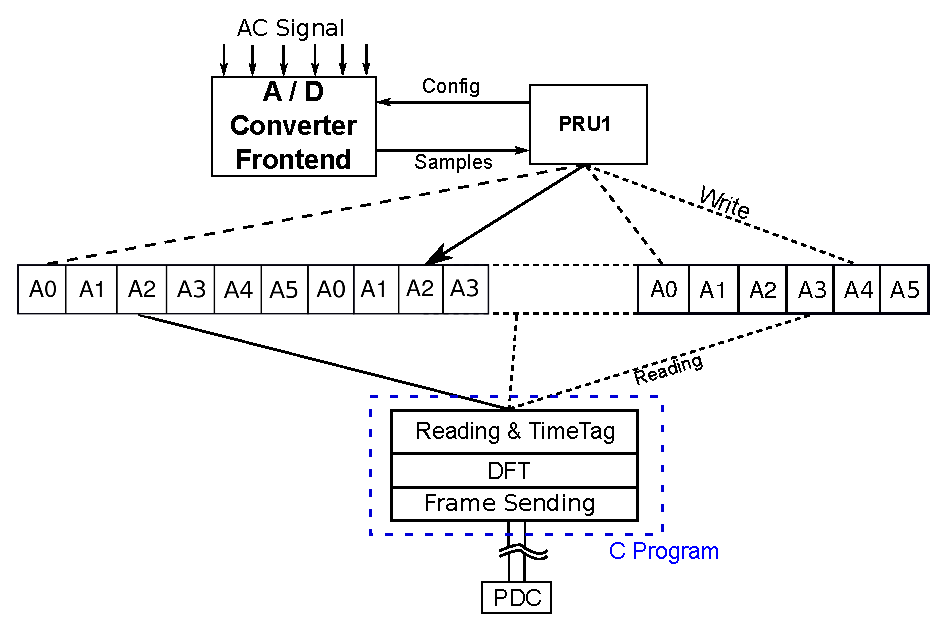
\includegraphics[width=\textwidth]{fig/sys_overview.eps}
	\caption{Overview of implementation}
\end{figure}

The implementation being described is a synchronized operation of three independent asynchronous subsystems: PRU, ADC and ARM core.
\begin{itemize}
	\item ARM side C program is written which configures PRU and uploads a binary file in to the PRU(1). PRU binary files does three task:
	\begin{enumerate}
		\item Configure ADC, with 
		\begin{itemize}
			\item Enables 6 channels by writing to \texttt{STEPCONFIGx}
			\item Configures Open Delay (\texttt{OpD}) = 0, by writing zeros to \texttt{STEPDELAYx} register  
			\item Sample delay (\texttt{SaD}) = 0 
			\item Sample Averaging (\texttt{SAvg}) = 1  by writing ones to  \texttt{STEPCONFIGx} registers and 
			\item Timer delay [\texttt{Tmr}]= 156250 ns
			\item \texttt{Mode} = continuous 
		\end{itemize}
		\item Define the bank to be used as buffer and size of buffer
		\item Parse the data received from FIFO buffer (of ADC) in to the ring buffer. 
	\end{enumerate}
	\item 6 ADC channels are enabled and the sampling rate is set to 128 samples/cycle/channel (using \texttt{Tmr} delay). the OpenDelay and Sample Delay are kept zero because our signal strength is enough. Timer delay is configured to $ \frac{1}{128 * 50} = 156250 ~ns $.
	\item In continuous mode the buffer is defined as ring buffer and the   buffer length is kept $ 128 * 6 = 768 * 2 = 1536 $. buffer length is kept double for reading and filling the buffer in Ping-Pong fashion.  
	\begin{figure}[h]
		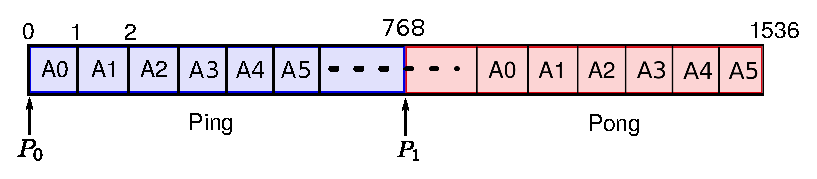
\includegraphics[width=\textwidth]{fig/ring_buffer.eps}
		\caption{Ring Buffer length and Ping Pong depicted}
		\label{fig:rb_pp}
	\end{figure}
	\item C program after uploading the bin file, sets the execution bit, This initiates the PRU execution, which signals ADC to start sampling with given configuration. PRU continuously fetches the the data from the output FIFO register of ADC and puts it in to ring buffer \textit{continuously} in sequential order of enabled channels [ \texttt{A0 A1 A2 A3 A4 A5 A0 A1.....A4, A5}].
	\item On the ARM side C program creates two pointers and using Ping Pong method over ring buffer reads the ADC samples in chunks. Brief description of how this works is described below and see Fig: \ref{fig:ping_pong}.
	\begin{itemize}
		\item[--] A buffer of double size then the target size is created (here of 1536 words) and two pointer  \texttt{P0} and \texttt{P1} are created, which points to the start and the middle of the buffer respectively. [ Step - 1 ]
		\item[--] Out of two pointer one works as \texttt{write head} and other as \texttt{read head}. So P0 keeps the track of number of ADC samples parsed in the buffer. [ Step-2 ]
		
		
		\begin{figure}
			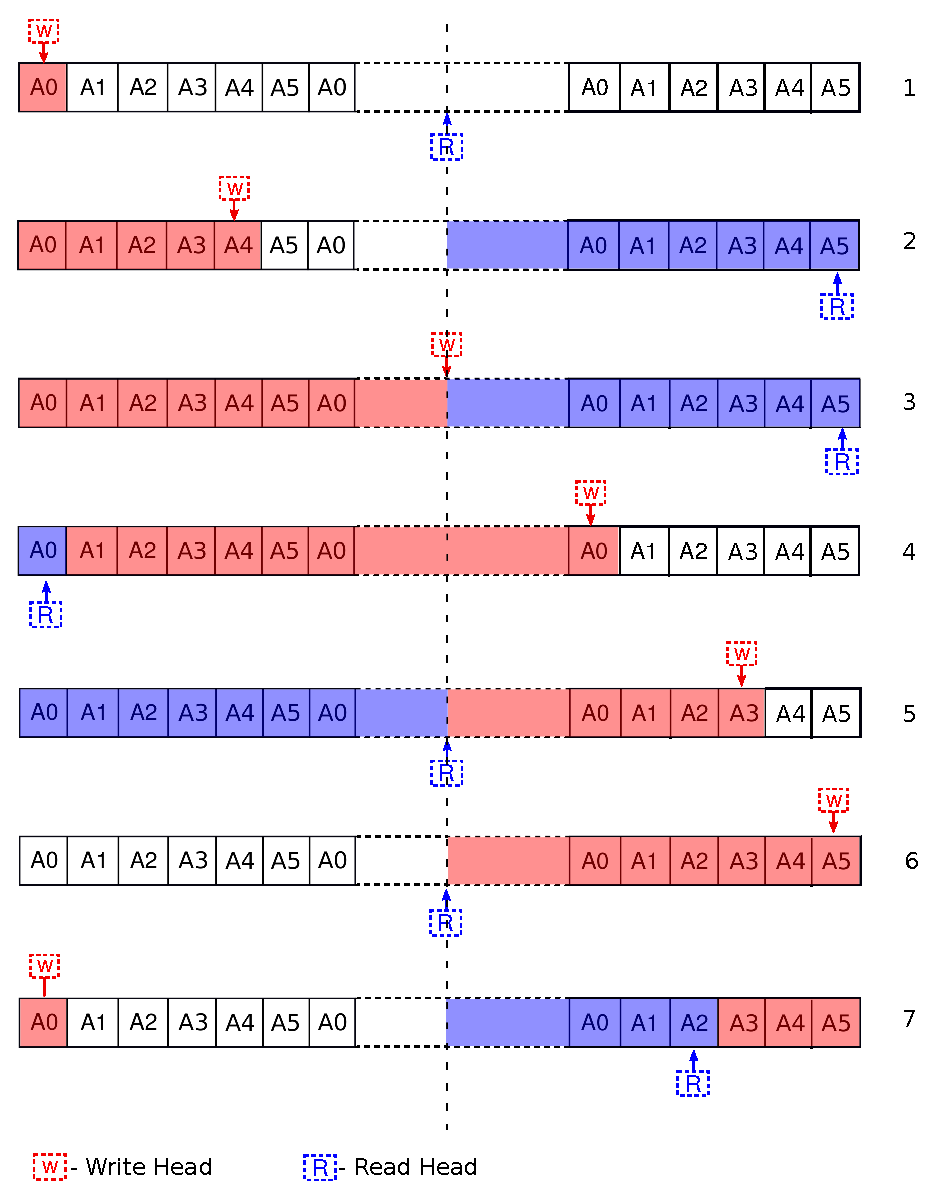
\includegraphics[width=\textwidth]{fig/ping_pong.eps}
			\caption{Ping-Pong Process Visualized}
			\label{fig:ping_pong}
		\end{figure}
		
		
		\item When P0 (write head) reaches 768 samples (128* 6, one whole cycle of all channels), pointers are swapped, P1 becomes the write head and P0 becomes the read head and goes to the beginning of the buffer and starts reading, while write head (pointer P1) continuous to write samples into buffer [ Step-3 ]
		\item Read operation is faster then write ( as PRU has to wait for the samples to arrive depending upon the sampling rate). Read head reaches the middle while P1 is still writing the samples. [ Step-5 ]
		\item After reaching the end of buffer, pointers are again swapped, P1 again becomes the read head and P0 Write head, which starts reading from the middle and the write goes to the beginning of the buffer and starts filling the samples. [ Step-6 ]
		\item From this point it is same as the beginning and the whole cycle repeats. [ Step-7 ]
	\end{itemize} 
	\item This way C program keeps on toggling between two buffers and there by allowing for concurrent reading and writing operation
	\item A visual depiction of the Ping-Pong process described above is show in the Fig: \ref{fig:ping_pong}
\end{itemize}

\begin{figure}[h]
	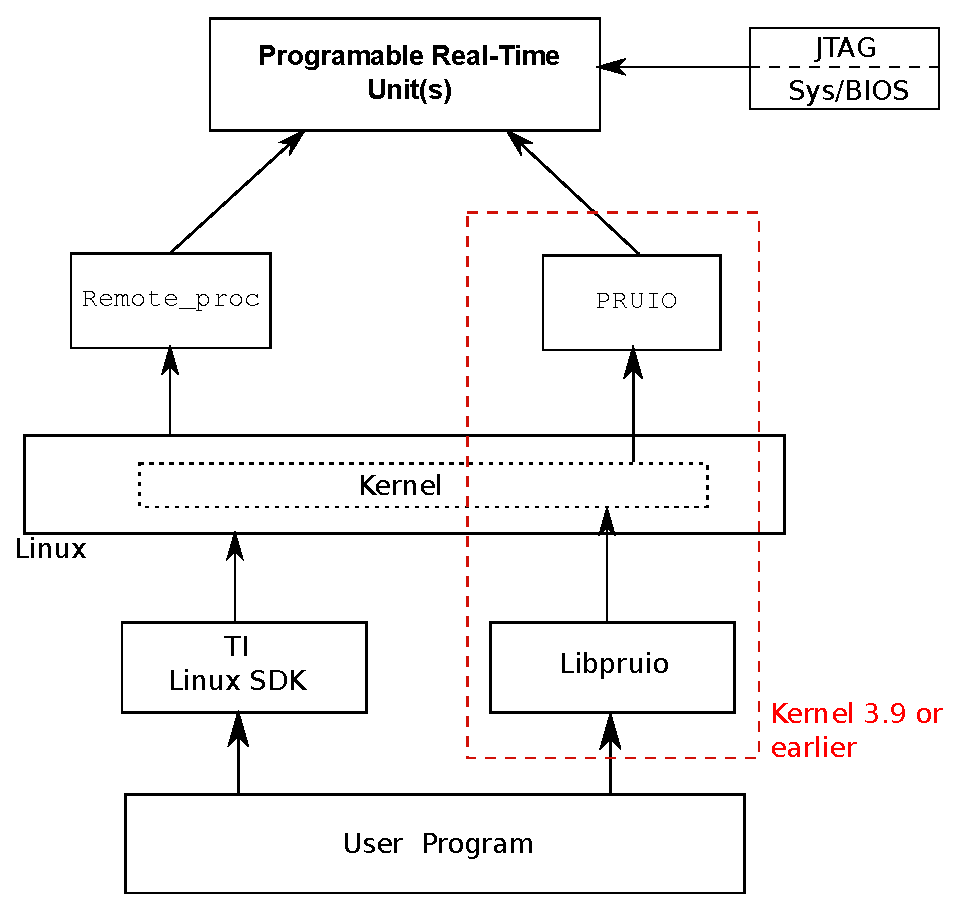
\includegraphics[width=\textwidth]{fig/PRU_config.eps}
	\caption{PRU Configuration Methods}
	\label{fig:pru_config}
\end{figure}

\subsection{PRU Configuration}
There are several way to configure PRUs, depending upon the kernel version, Operating System and the mode of connection.
\begin{enumerate}
	\item PRUIO - PASM 
	\item Remote\_Proc
	\item Direct firmware loading via JTAG
\end{enumerate}

A visual overview of different way of accessing PRUs is show in Fig: \ref{fig:pru_config}.
\subsubsection{PRUIO}
 For Kernel version older then 3.9 PRUIO kernel module is used which uses a Device Tree Overlay. Device trees are a way to describe Hardware in system, their memory address, their port number or there function. A good example of it would be how UART is described in the system. Device tree enables addition of new hardware in run-time from User Space, in the kernel architecture. 
 
 Usually ``Board File" is used in kernel package to describe a hardware of specific embedded system, but given the huge number of ever increasing ARM based devices it was impossible to incorporate all the boards' file in to main Kernel. So Linus Torvalds \cite{DThist} suggested the use of DT, to simplify the kernel maintenance and up-keeping while providing complete flexibility to describe their processor (something that was already being done by PowerPC manufacturers). So, usage of kernel module and Device Tree enables us to configure PRUs and use them. it maps PRU's register memory address to our use space addresses and enables direct access to them. 
 
 A library  called as \textbf{libpruio} \cite{libpruio} is used here, for convenience and rapid development. The library provides C and FreeBasic API's for accessing and configuring ADC, GPIO and PWM modules. It uses converts user C code to Assembly Language via PASM and uploads it to the respective PRUs. A detailed explanation along with program listing is given in Appendix-1.
 
 \subsubsection{Remote\_Proc}
 Modern SoCs have multiple processors and processor cores on them in asymmetric multiprocessing (AMP) configuration. which may be running different instances  of operating system, whether it's Linux or any other flavor of real-time OS  . So to enable single kernel to control all those remote processors while abstracting hardware differences and there by reducing the duplication of code \textit{Remote Processor Framework} is used \cite{remoteproc}.
 
 Here in case of AM3358, Remoteproc acts as a framework that allows the ARM host processor(s) to load firmware into PRU cores, start the PRU cores, stop the PRU cores, and configure resources that the PRUs might need during their execution (such as configuring the PRUSS INTC module and providing shared buffers in DDR memory for message passing).

\subsubsection{Direct Loading}
TI provides different development mediums for it's products, For  AM335x also, there existed - Sys/BIOS support, TI Starterware support and Ti Processors-SDK support. out of which Sys/BIOS ad Starterware are a non-OS solution which posses bare minimum driver support in form of modules, which is very useful in rapid development and due to no OS, latency was brought down to bare minimum.
\begin{figure}[h]
	\centering
	\includegraphics[width=\textwidth/2]{fig/bbb_jtag.jpg}
	\caption{A BeagleBone connected Via Ti's Hawk JTAG}
\end{figure}

Efforts were made to utilize Sys/BIOS initially for the project but it had become obsolete and was being phased out by TI, which resulted into poor support for relatively newer processor like AM3358. Then efforts were made for using TI-Processor SDK as well, but it required a special ARM \texttt{TMDSEMU100v2U-20T} JTAG-extension header-connector which was not available and hence had to be dismissed. But in principal if one possesses the JTAG, TI-processors SDK can be a very competitive implementation compared to a Linux based implementation, due to real-time capability, direct access to PRU and optimized device drivers by Ti itself.


\subsection{Time stamp, GPS interfacing and Data Processing }
As seen in the previous section, data is read in chunks each chunk has 768 samples which consists of 128 samples from all 6 channels. This makes it more convenient to handle and process the data. Using GPS for time reference was aimed but due to hardware interfacing issues, GPS could not be interfaced instead Network Time Protocol (NTP) is being used for time-keeping. Time stamp for each frame is stored on the first sample of the frame written to the buffer.

\begin{itemize}
	\item DFT window of 2 cycle, 256 samples is chosen for better frequency resolution, and then blackman-harris window function is applied to smooth out the samples.
	\item After applying blackman-harris window, simple FFT is done and frequency is extracted from the beans. 
	\item After extracting the frequency, amplitude and angle is extracted..
\end{itemize} 

\subsection{Communication}

After DFT is calculated we have the necessary information to send. Structure of the frame depends upon the configuration and specification of the PMU. Hence as per standards a configuration frames should be communicated by PMU to PDC, which lists following things:
\begin{enumerate}
	\item Time Format 
	\item Number of phasors
	\item Format of the phasor (rect or polar)
	\item Frequency
	\item Number of digital status, if any
	\item Error Bit
\end{enumerate}

The frame configuration used by our device is as show below:
\begin{itemize}
	\item Device ID
	\item TimeTag 
	\item 6 phasor entity 
	\item Frequency
\end{itemize}

Once the device is turns ON, it establishes a communication to the PDC, by communicating a acknowledgment string once that is communicated PMU starts sending the data to the PDC. Currently PDC is implemented by us just accepts the data and writes to file rather then parsing in to a database, it receives the data over ethernet via TCP/IP, separates each information from frames and writes it to a file. For evaluation purposes the communication delay, sampling delays and reporting time are computed. This is done by computing the time difference between two frame received, by measuring time difference between two time tags of consecutive data frames and by measuring the time taken for the data packets to be received. 

\section{Challenges Faced}
There were several challenges faced and solved which are worth mentioning for others who might embark on this path and face it

\begin{itemize}
	\item GPS module interfacing
	
	NavSync CW-12 TIM GPS module was chosen to provide time to the device. It was connected to the GPS antenna, power was provided and sometimes it lock to 3 Satellites but it fails to get interfaced via serial ports. It has UART \texttt{RxD} and \texttt{TxD} , \texttt{GND} and \texttt{Vcc} pin out.  For configuring it a utility called \textit{WinOnCore} is provided for Windows bases systems. GPS module's UART is connected to PC via FTDI R232L serial to serial convert IC and sends messages to the utility. The problem is while grounds of both system (GPS receiver and PC) are separate WinOnCore fails to communicate with the module but upon looking in "serial terminal" some random message are being thrown by the module. Yet, the moment ground of device is connected to the ground of PC, even those messages stop working. This is a very unusual behavior, Efforts with different power supply, with a new GPS receiver, with different USB to serial converter but all efforts are futile yet.
	
	\item DFT computation Time 
	PMU's DFT requirements are not so complicated and the computational power at hand is also limited hence simple brute force DFT is tried. but it was taking huge time to compute on ARM processor. Initial latency observed was as high as $4.23 ~ms$/channel. Which was optimized by implementing \texttt{look-up tables} and by removing the \texttt{divisions} and putting multiply instead. Now each DFT operation typically  takes 240 to 400 $\mu s$. 
	
%	\item Overlapping ADC samples 
	

\end{itemize}
\chapter{Results and Discussion}
The device has been designed completely from scratch. So, to make it standard compliant it is necessary to test all its aspect and keep them well below the limit so that final results are well within the stipulated guideline. Hence, here qualitative and quantitative results are presented which include computation latency, reporting rate \& variation, ADC response(s) and amplitude \& frequency estimation.

\section{Frequency Computation}
\subsection{Steady State Nominal Frequency Operation}
First, we will see the frequency response of the device. First nominal frequency test was done, where device was given 50 Hz nominal frequency.
\begin{figure}[h]
	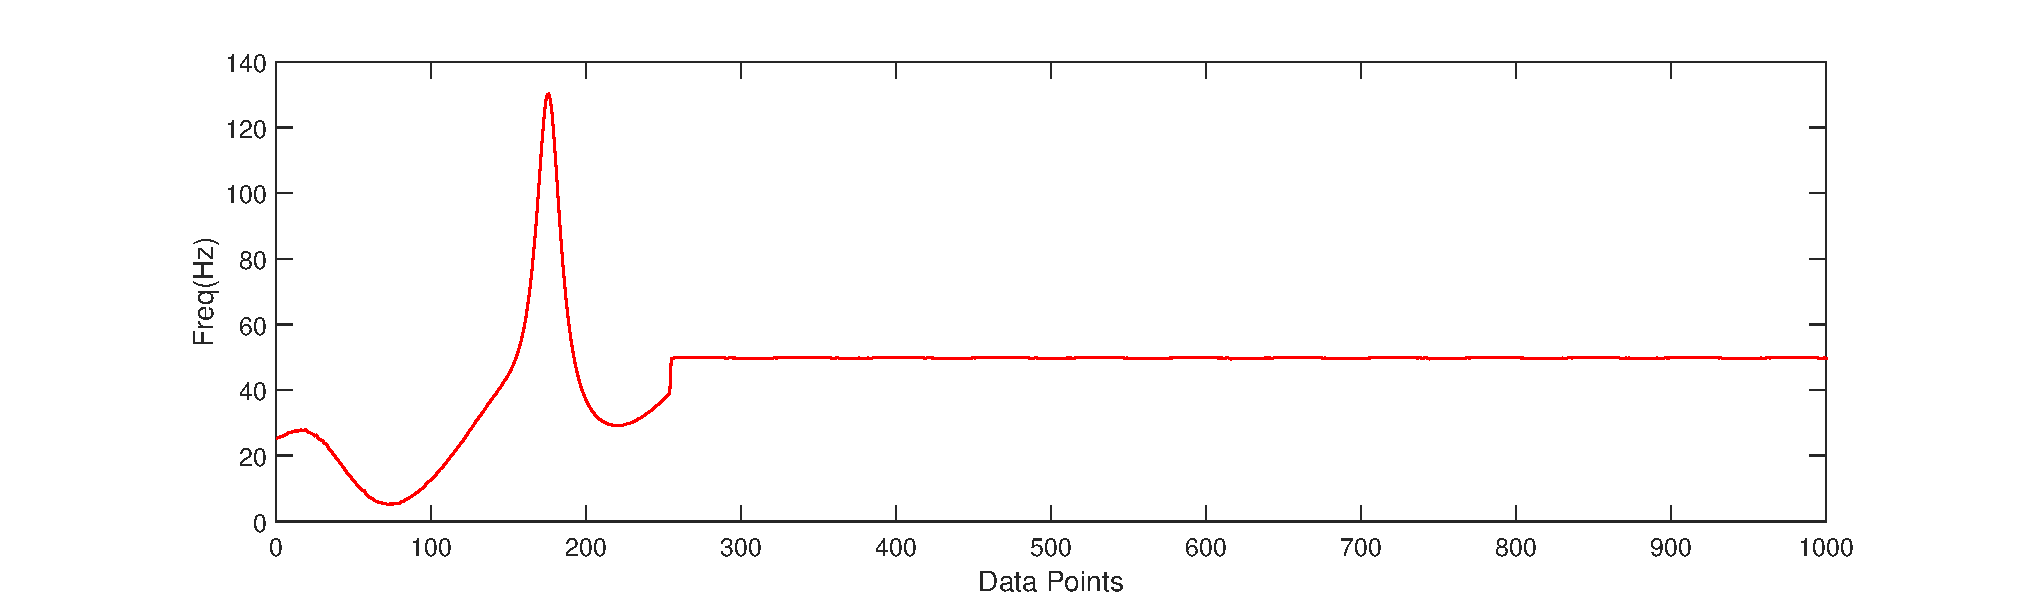
\includegraphics[width=\textwidth]{fig/50Hz_freq_1000samples.eps}
	\caption{Deice Frequency Response to 50 Hz sine input}
	\label{fig:50hzlongdata}
\end{figure}

In Fig: \ref{fig:50hzlongdata} shows response to an input signal of fundamental frequency 50 Hz. As it can be seen the initial portion has irregularities because of the moving window not being completely filled. length of moving window is 256 samples, hence for first two cycles the window is filled with zeros, which slowly gets filled and then device settles to a final steady state position.

\begin{figure}[h]
	\includegraphics[width=\textwidth]{fig/50Hz_freq_closeup.eps}
	\caption{Zoom-in plot of steady state frequency reading}
	\label{fig:50Hzcloseup}
\end{figure}


If the end part (i.e. steady state, for the device) is zoomed in then oscillation and noise can be seen in the reading as show in Fig: \ref{fig:50Hzcloseup}. It is important to note here, that the plot shown here are instantaneous frequency given by the device, as a qualitative representation of each DFT computation at each point on wave, instead of the averaged value over a cycle. Error was computed on non-averaged instantaneous values and following results weere obtained as show in Fig: \ref{fig:50Hz error}.

\begin{figure}[h]
	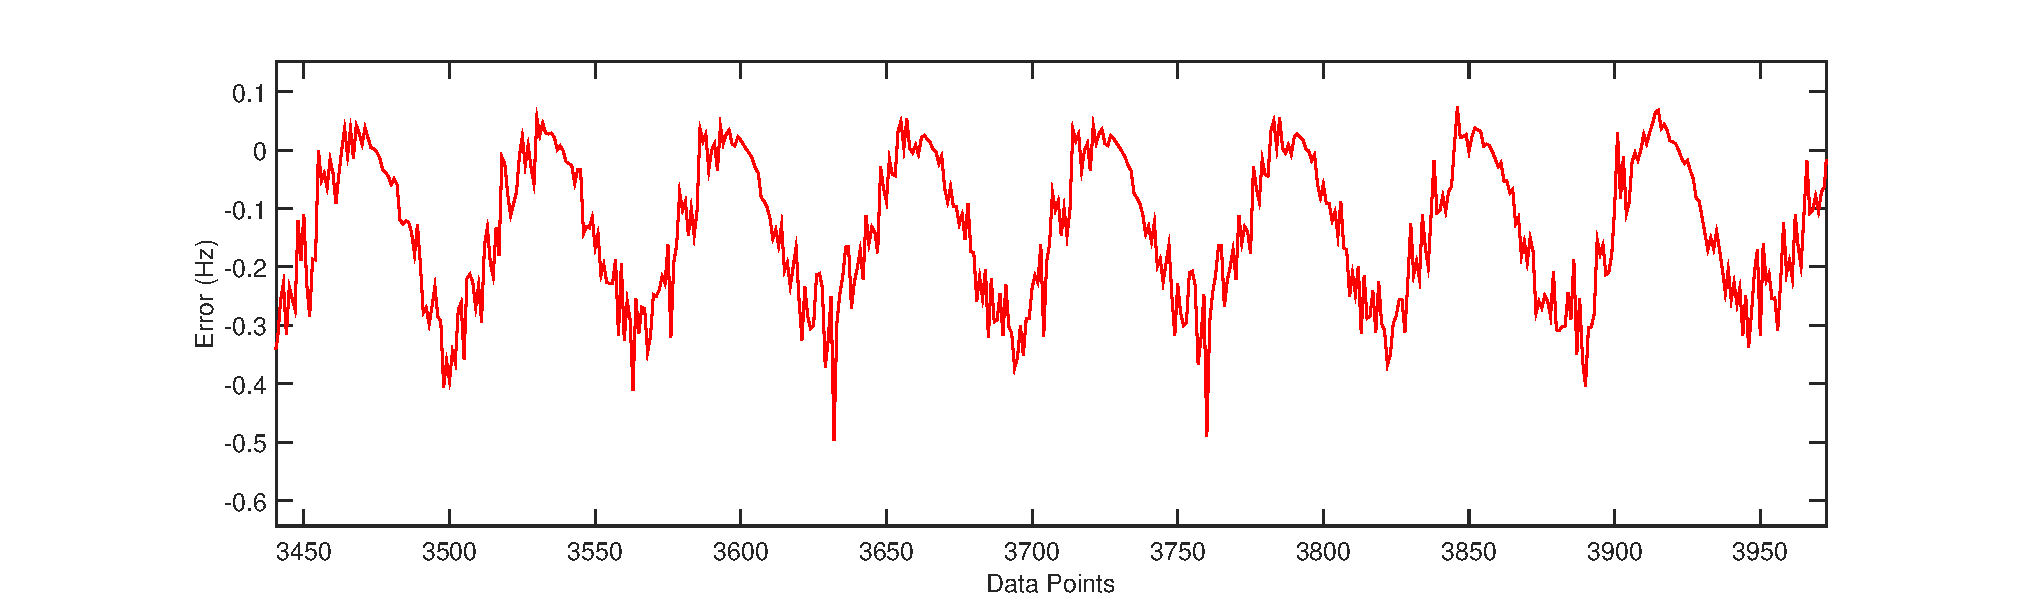
\includegraphics[width=\textwidth]{fig/50Hz_freq_error_closeup.eps}
	\caption{Error Plot for 50 Hz input}
	\label{fig:50Hz error}
\end{figure}
For verifying the results coming from the developed PMU, a simulation program was written, same 256 sample moving window DFT was implemented and same nominal frequency input was given which resulted in to output which is show in Fig: \ref{fig:50Hz simulation}. It is important to note here that though by appearance simulation result \emph{profile} looks worse than the actual results obtained from hardware but in reality they are not, it is due to the the high degree of precision. Here as it can be seen in Fig: \ref{fig:50Hz simulation} range of values is  \texttt{Max:49.99999999995302} to \texttt{Min: 50.00000000005302}, which can practically be considered 50.0 Hz. 
\begin{figure}[h]
	\includegraphics[width=\textwidth]{fig/50Hz_simulated.eps}
	\caption{Simulation Output at 50 Hz}
	\label{fig:50Hz simulation}
\end{figure}
   
\subsection{Steady State Off-nominal Frequency Behaviour}
Qualitatively ability to compute/detect the off-nominal frequency effectively is an important factor. So here different frequency values (i) 50.2 Hz (ii) 50.5 Hz (iii) 49.8 Hz \& (iv) 49.5 Hz are considered for evaluation of device. 

\subsubsection{49.5 Hz Operation}
\begin{figure}[h]
	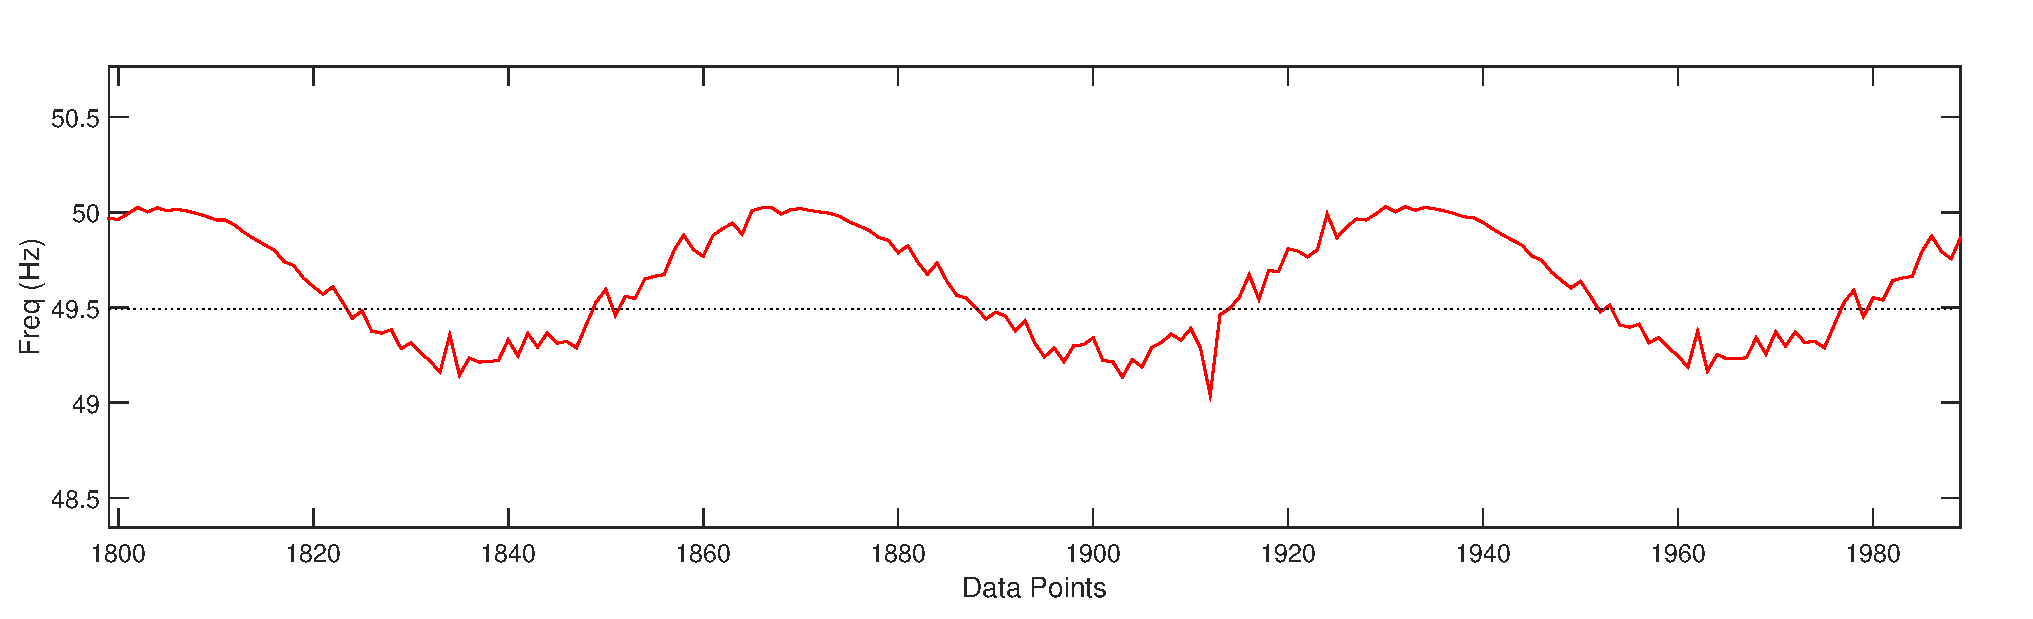
\includegraphics[width=\textwidth]{fig/495Hz_freq_reading.eps}
	\caption{Device reading at 49.5 Hz}
	\label{fig:49.5Hz operation}
\end{figure}
For the off-nominal frequency operation a guide line is drawn on the plot and as it can be seen, that PMU follows perfectly the marker. This is raw data if it is averaged out then it would accurately report the input wave frequency.Range of readings was \texttt{Max:50.12} to \texttt{Min:48.807} Hz

\subsubsection{49.8 Hz Operation}
\begin{figure}[h]
	\includegraphics[width=\textwidth]{fig/498Hz_freq.eps}
	\caption{Device reading at 49.8 Hz}
	\label{fig:49.8Hz operation}
\end{figure}
Fig: \ref{fig:49.8Hz operation} show the operation of PMU at 49.8 Hz input signal. It can be observed that the operation is quiet poor on off-nominal frequency.

\subsubsection{50.2 Hz Operation}
\begin{figure}[h]
	\includegraphics[width=\textwidth]{fig/502_Hz_freq.eps}
	\caption{Device Reading at 50.2 Hz}
	\label{fig:50.2Hz operation}
\end{figure}
As it can be seen in Fig: \ref{fig:50.2Hz operation} PMU was giving poorer responses. Overall average frequency reported was 50.05 Hz with samples varying in range of \texttt{Max:50.35 Hz} to \texttt{Min:49.99 Hz}.


\subsubsection{50.5 Hz Operation}
\begin{figure}[h]
	\includegraphics[width=\textwidth]{fig/505_Hz_freq.eps}
	\caption{Device reading at 50.5 Hz}
	\label{fig:50.5Hz operation}
\end{figure}
Comparison of Fig: \ref{fig:50.5Hz operation} with previous figures, like Fig: \ref{fig:50.2Hz operation}, Fig: \ref{fig:49.8Hz operation} and Fig: \ref{fig:49.5Hz operation} it can be clearly observed that there is a deterioration in the profile and it is well drifted away from the standard result.The deviation observed was \texttt{Max:50.23 Hz} to \texttt{Min:50.16 Hz}.
%%
%\subsection{Error Plot}
%A plot of error existing in the each test case is plotted to give an overview of %error(s) in the result(s).  

%===========================================================================

\section{Phase Computation}
\subsection{Steady State Nominal Frequency Phase results}
 
\begin{figure}[h]
	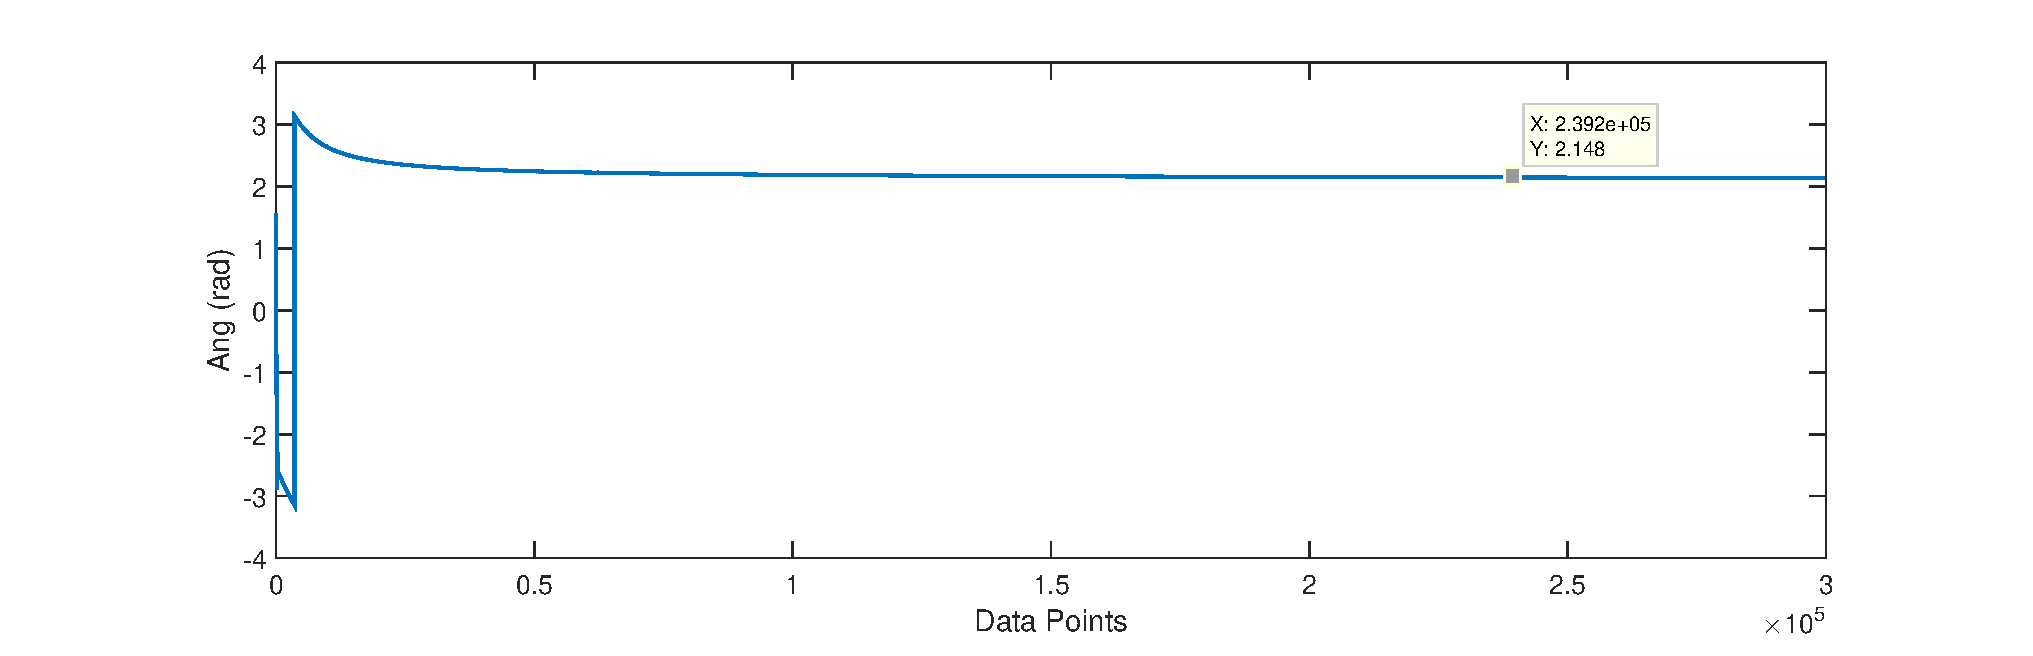
\includegraphics[width=\textwidth]{fig/50Hz_angle.eps}
	\caption{Phase angle at 50 Hz}
	\label{fig:50Hz ang}
\end{figure}
Fig: \ref{fig:50Hz ang} shows the phase reported by the device for a 50Hz input signal. And as expected it settles to a steady state value this proves that there exist zero relative angular velocity between the reference frame and the input signal. Now we will see angle reporting performance for other few frequencies.

\subsection{Steady State Off-nominal Frequency Phase results}
Contrary to the steady state 50 Hz operation, in case of off nominal frequency operation the angle of phasor keeps changing (due to the leakage effect) either increasing or decreasing depending upon the relative frequency). 
\subsubsection{49.5 Hz Operation}
\begin{figure}[h]
	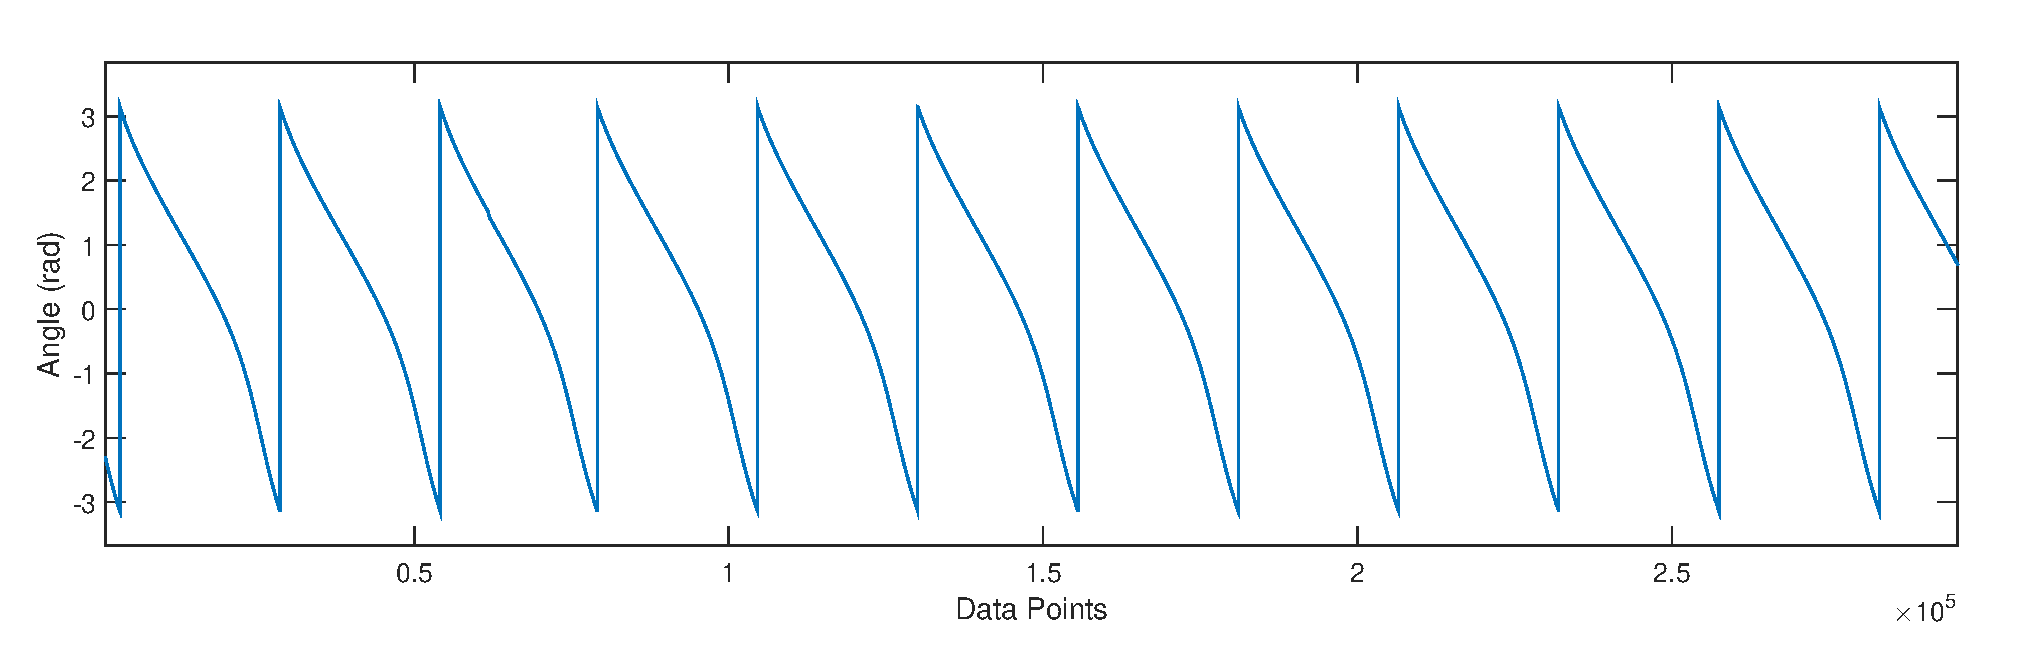
\includegraphics[width=\textwidth]{fig/495Hz_ang.eps}
	\caption{Phase angle of 49.5 Hz input signal}
	\label{fig:49.5Hz ang}
\end{figure}

\begin{figure}[h]
	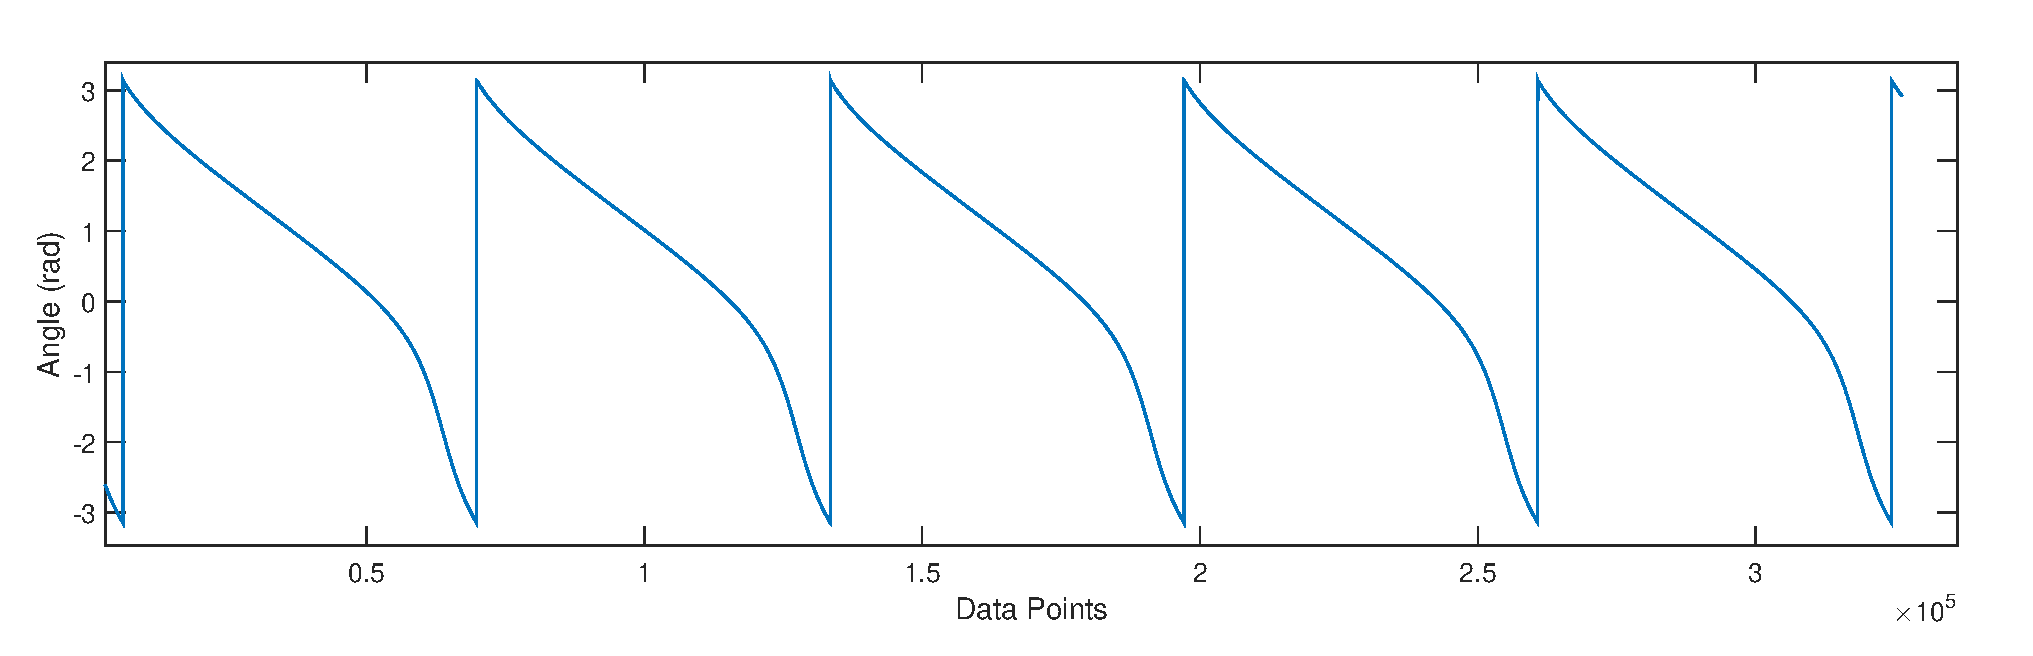
\includegraphics[width=\textwidth]{fig/498Hz_ang.eps}
	\caption{Phase angle of 49.8 Hz input signal}
	\label{fig:49.8Hz ang}
\end{figure}
 
Representative plots of two phasors at 49.5 Hz and 49.8 Hz are presented here. And we can see the \emph{angle wrap} taking place due to relative difference in angular velocity.

\subsubsection{Computation delay}
Completion of all computation and processing within given time limit is necessary. For 50 Hz system 20 ms is the time period within which whole process should be over. In this section we will see the latency involved in computation. Fig: \ref{fig:simpleLatency} shows the time taken by the program in computing DFT.

\begin{figure}[h]
	\includegraphics[width=\textwidth]{fig/simple_latency.eps}
	\caption{Normal computation latency}
	\label{fig:simpleLatency}
\end{figure}

As it can be seen from Fig: \ref{fig:simpleLatency}, time taken by the program is way below the threshold. There are peaks seen in-between, which are caused partly because of other OS services running in background and partly due to the C-program copying the new data from the PRU buffer to the RAM.   

\begin{figure}[h]
	\includegraphics[width=\textwidth]{fig/optimised_latency.eps}
	\caption{Compiler optimised latency}
	\label{fig:optimisedLatency}
\end{figure}
Fig: \ref{fig:optimisedLatency} shows latency of the DFT computation after compilation time optimization. Details about the runtime optimization and compilation optimizations are given in Appendix-B.


%\chapter{Chapter 4 Title}
\section{Chapter 4 Section 1}
\subsection{Subsection 1}
\section{Chapter 4 Section 2}

\begin{appendix}
\chapter{PRU-ADC implementation}

\chapter{OMAPL-137 implementation}

\end{appendix}


\bibliographystyle{IEEEtran}
\bibliography{reference1}
                                                                                                                 
\end{document}
